% Dieser Text ist urheberrechtlich gesch�tzt
% Er stellt einen Auszug eines von mir erstellten Referates dar
% und darf nicht gewerblich genutzt werden
% die private bzw. Studiums bezogen Nutzung ist frei
% Mai. 2007
% Autor: Sascha Frank 
% Universit�t Freiburg 
% www.informatik.uni-freiburg.de/~frank/
\documentclass{beamer}
% \documentclass[notes=only]{beamer}
\usepackage{pst-bar,pst-plot,pstricks-add}
\usepackage{graphics,graphicx}
\usepackage{pstricks,pst-node,pst-tree}
% \setbeameroption{show notes}
\setcounter{tocdepth}{1}

\setbeamertemplate{navigation symbols}{}
\beamersetuncovermixins{\opaqueness<1>{25}}{\opaqueness<2->{15}}
\usetheme{CambridgeUS}
\usecolortheme{seahorse}

\begin{document}
	\title{The max-min-hill-climbing algorithm}  
	\author[M. Bauer]{Michael Bauer}
	\institute[M.Sc. Comp. Science]{M.Sc. Comp. Science}
	\date{\today}


\begin{frame}
	\titlepage
\end{frame}

\section{MMPC}
	\begin{center}
		\begin{frame}
			\begin{center}
				\begin{figure}
					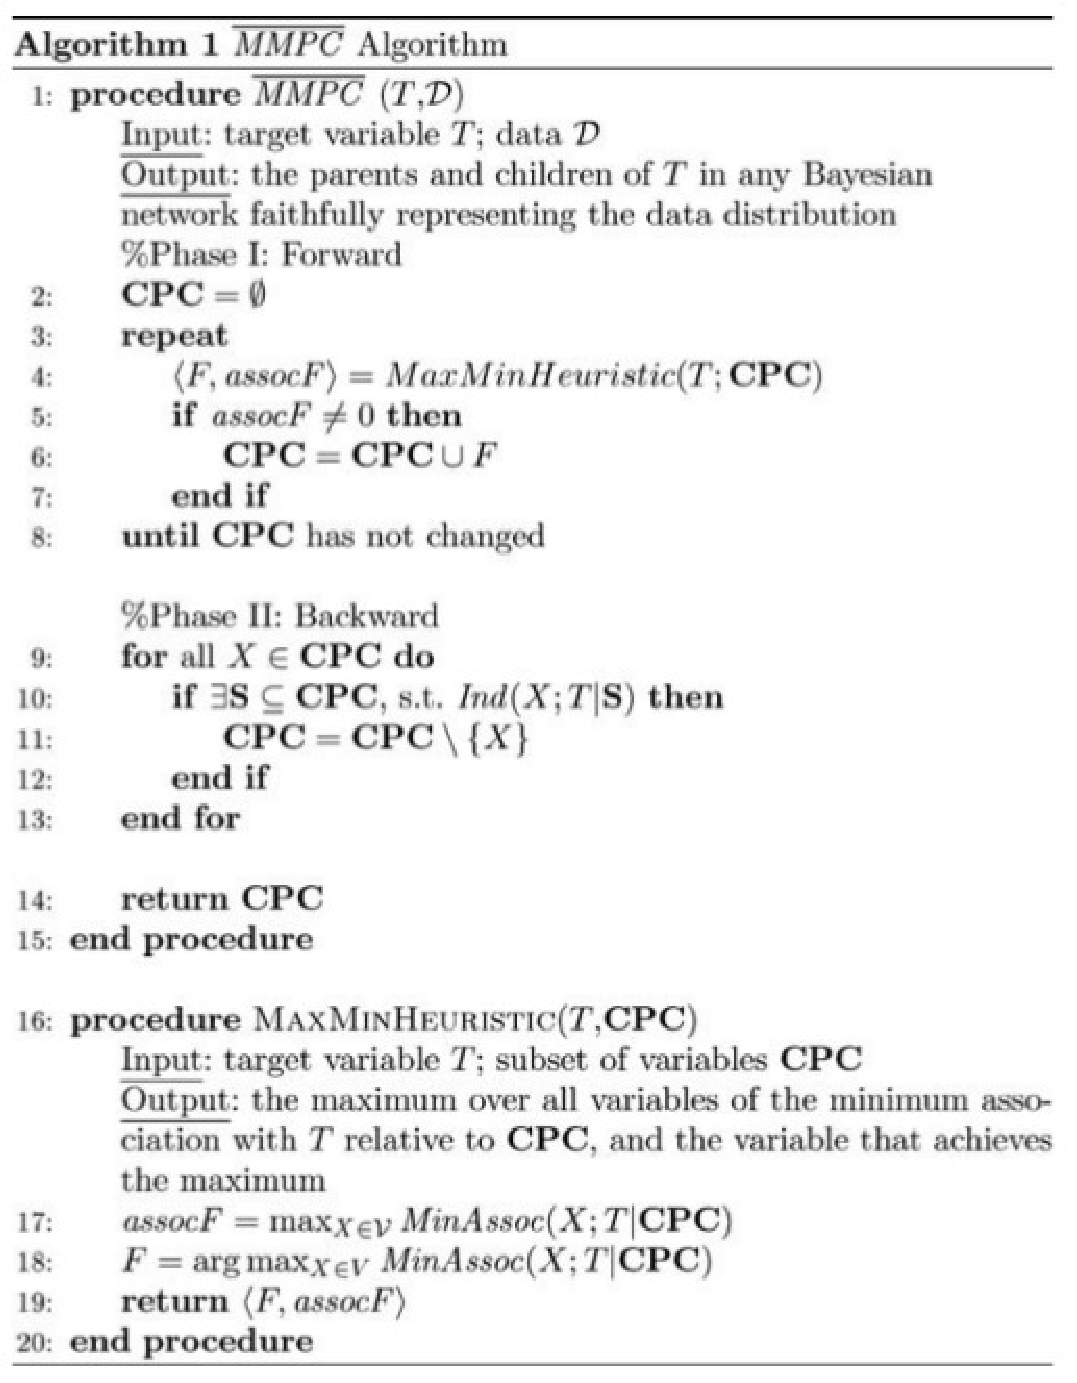
\includegraphics[scale=0.38]{img/mmpc_bar}
				\end{figure}
			\end{center}
		\end{frame}
	\end{center}

\section{Statistics}
	\subsection{Conditional Independence}
		\begin{frame}
			\begin{block}{Definition}
				% It is equivalent
				% 	\begin{equation}
				% 		Ind(X;T|\textbf{Z}) \Longleftrightarrow (Assoc(X;T|\textbf{Z}) = 0),
				% 	\end{equation}
				% where $Assoc(X;T|\textbf{Z})$ is the strength association (dependency) of $X$ and $T$ given $\textbf{Z}$. \\
				We define the minimum association of $X$ and $T$ relative to a feature subset $\textbf{Z}$, as
					\begin{equation}
						MinAssoc(X;T | \textbf{Z}) = \min_{\textbf{S} \subseteq \textbf{Z}} Assoc(X; T | \textbf{S}).
					\end{equation}
			\end{block}
		\end{frame}

% \section{Forward Phase}
% 	\subsection{How the algorithm works}
% 		\begin{center}
% 			\begin{frame}
% 				\begin{center}
% 					\begin{figure}
% 						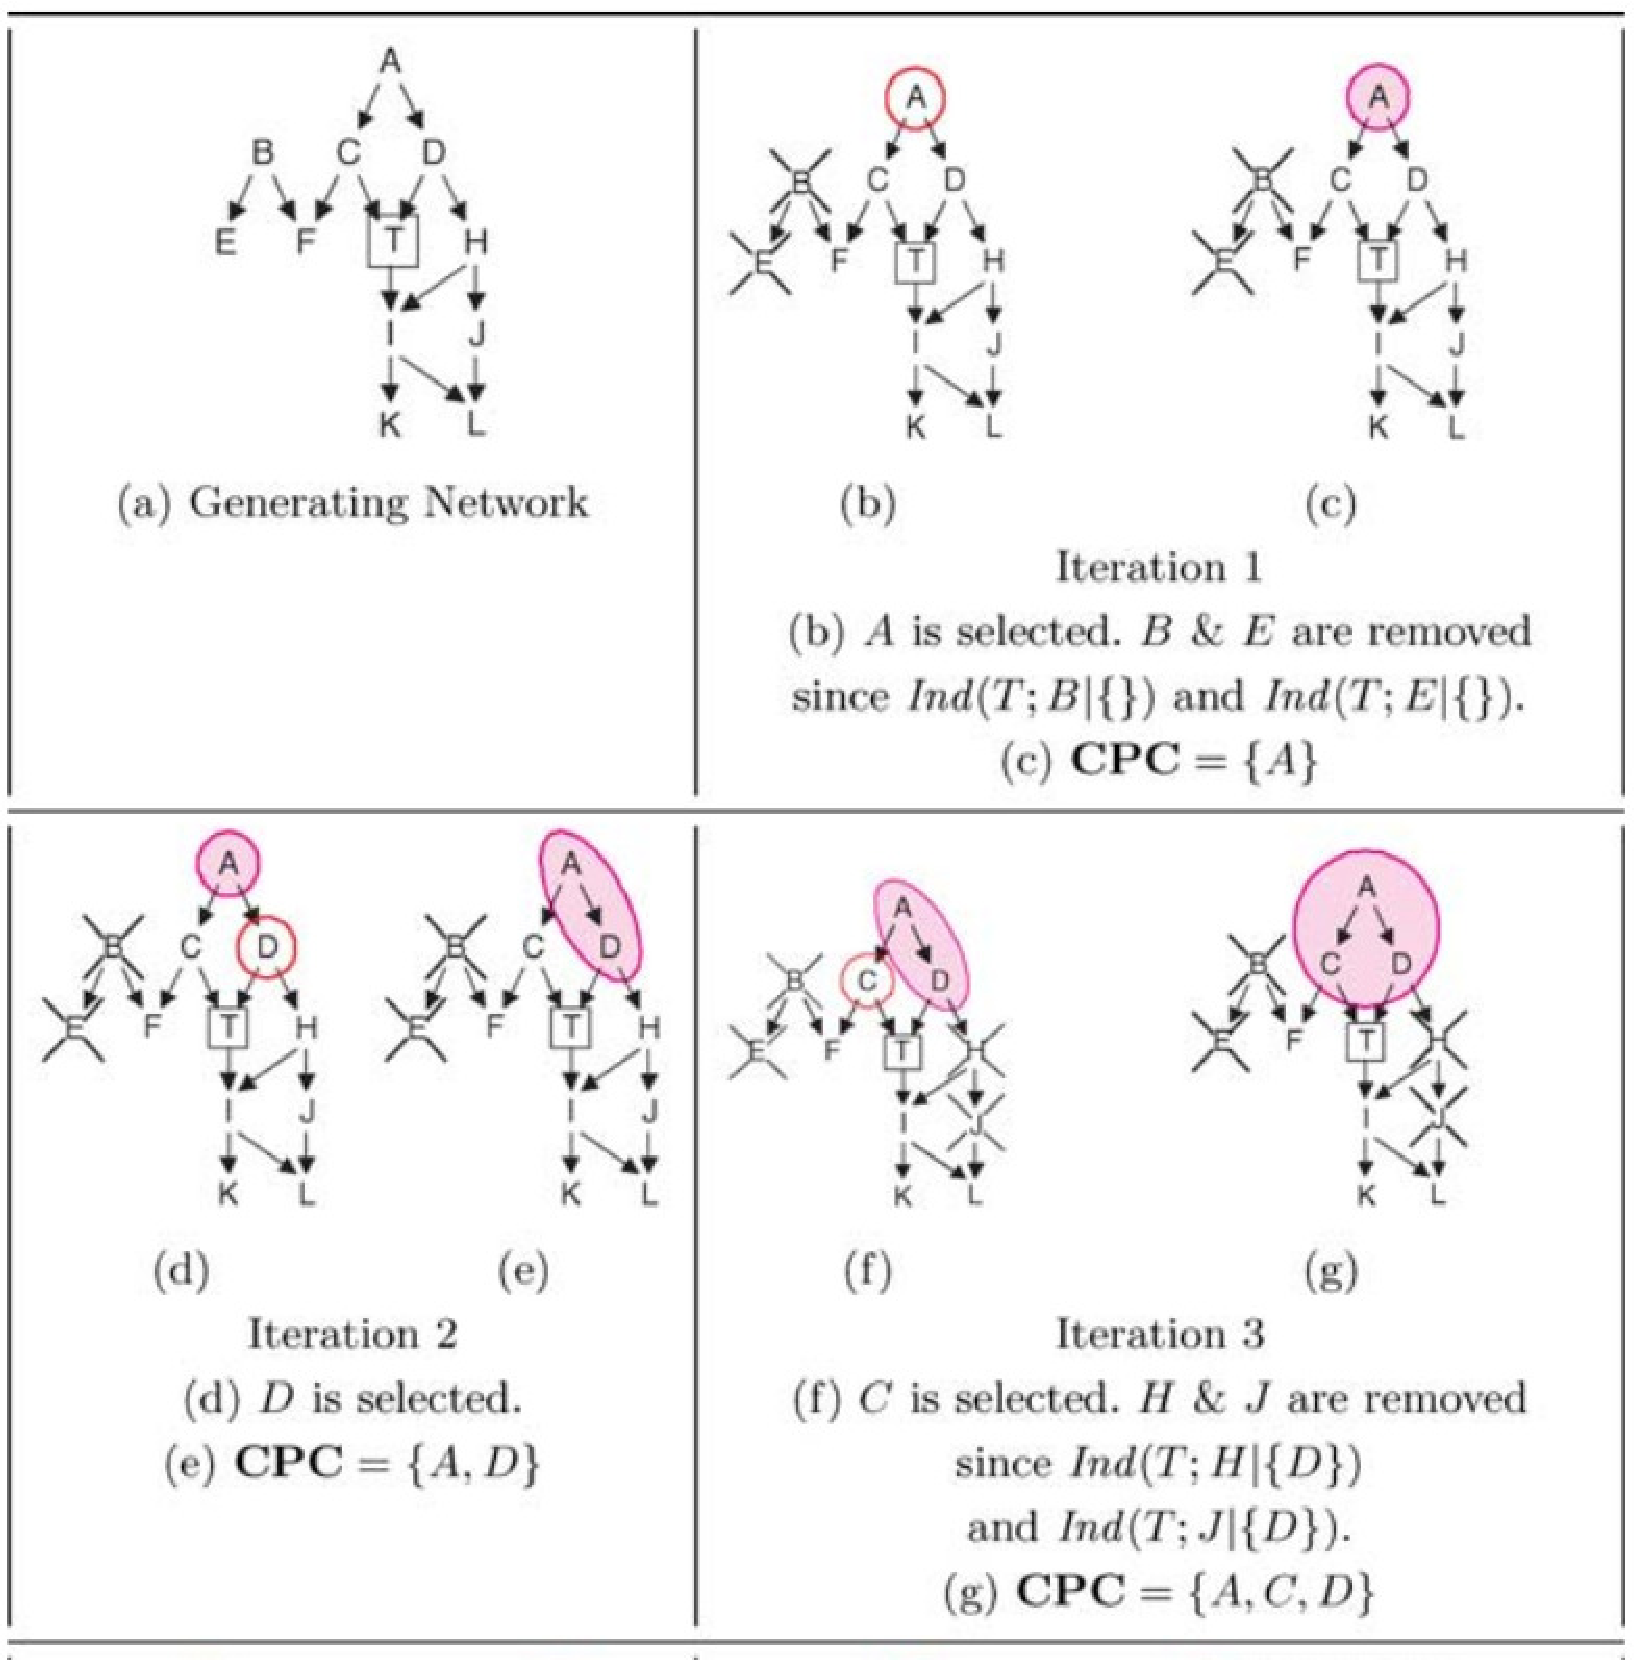
\includegraphics[scale=0.3]{img/example_part1}
% 					\end{figure}
% 				\end{center}
% 			\end{frame}
% 		\end{center}

\section{Statistics}
	\subsection{The $G^{2}$ value}
		\begin{frame}
			\begin{block}{Definition}
				We calculate the $G^{2}$ value under the nullhypothesis of the conditional independence of $Ind_{P}(X_{i},X_{j}|\textbf{X}_{k})$ holding. Then, the $G^{2}$ value is defined as:
				\begin{equation}
					G^{2} := 2 * \sum_{a,b,c} S^{ab\textbf{c}}_{ijk} * ln \left( \frac{S^{ab\textbf{c}}_{ijk}*S^{\textbf{c}}_{k}}{S^{a\textbf{c}}_{ik}*S^{b\textbf{c}}_{jk}} \right),
				\end{equation}
				where $S^{abc}_{ijk}$ is the number of times in the data where $X_{i} = a$, $X_{j} = b$ and $\textbf{X}_{k} = \textbf{c}$. We define in a similar fashion $S^{ac}_{ik}$, $S^{bc}_{jk}$ and $S^{c}_{k}$, respectively.
			\end{block}
		\end{frame}

	\subsection{Query the graph}
		\begin{center}
		\begin{frame}
			\begin{center}
				\begin{figure}
					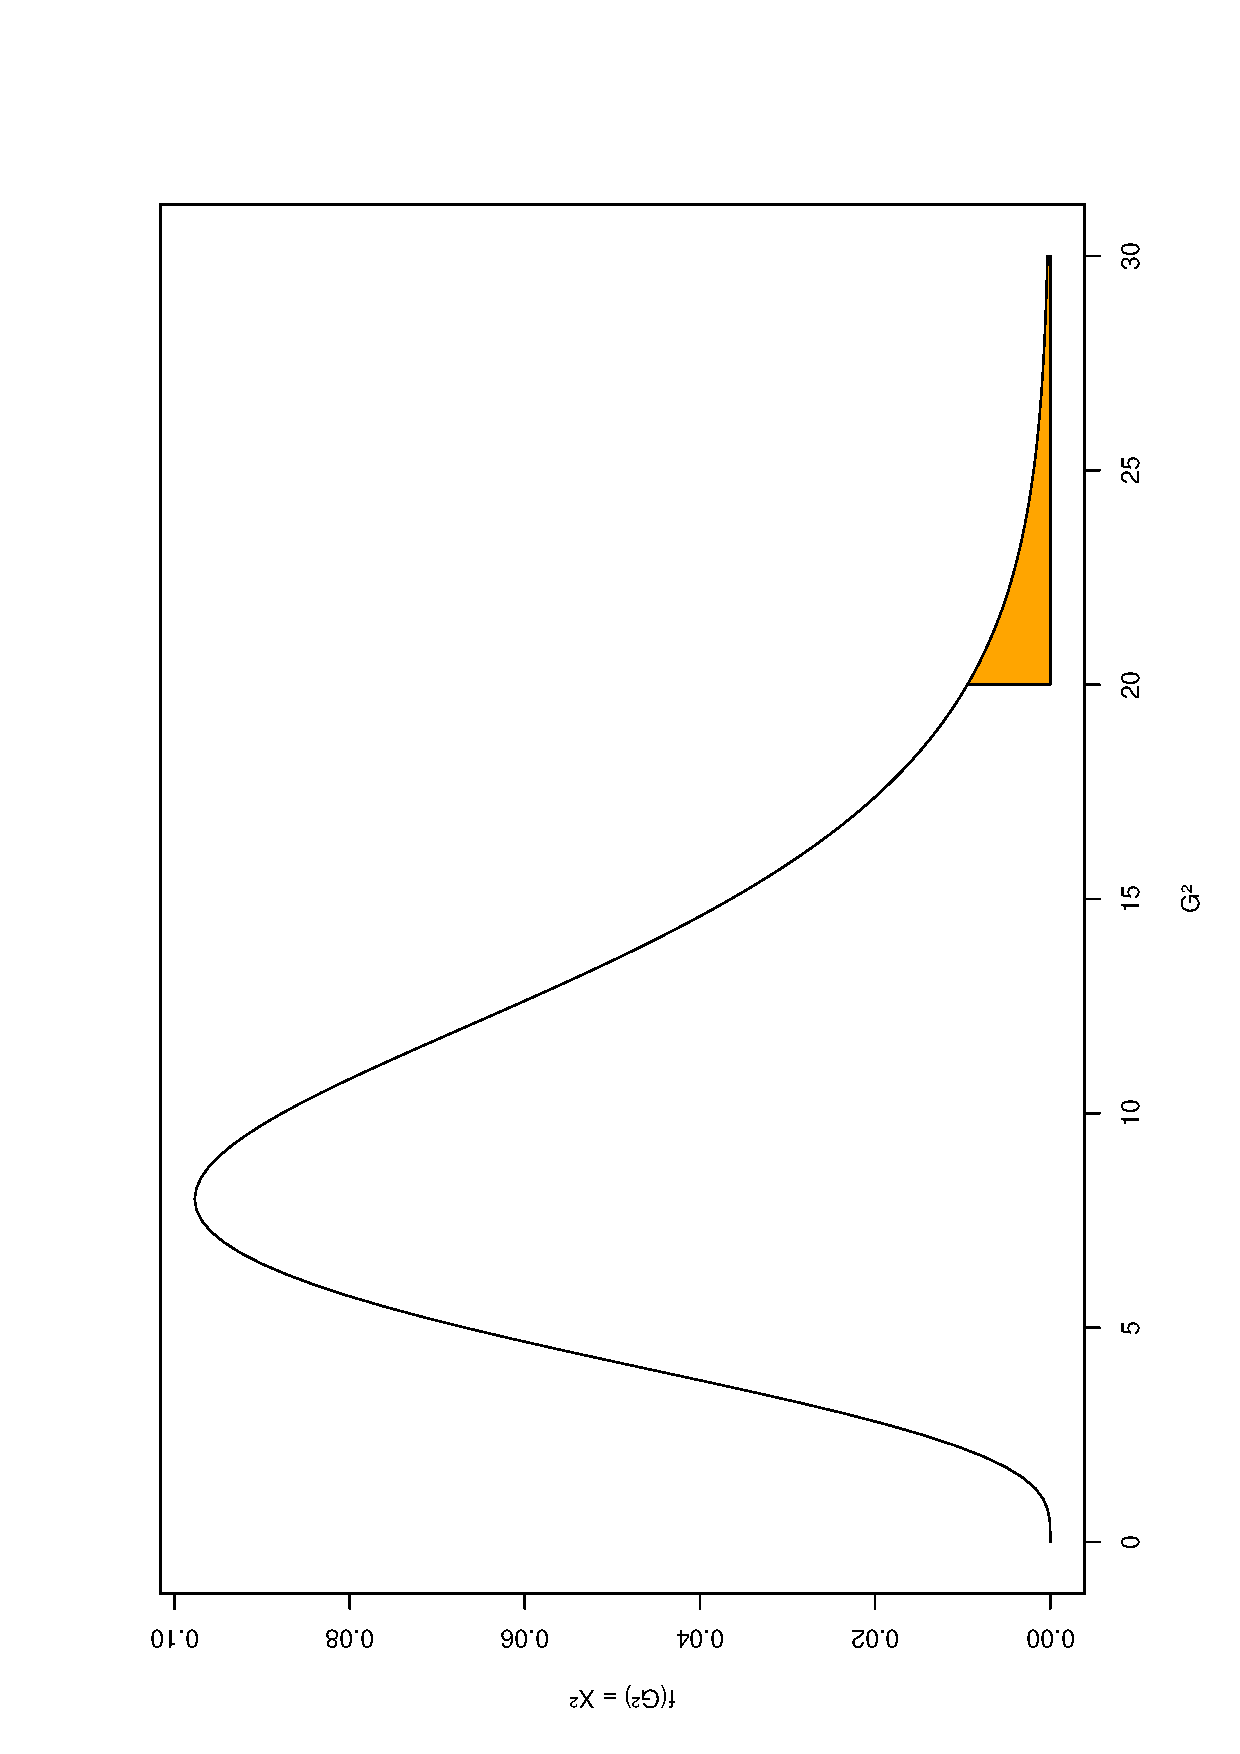
\includegraphics[scale=0.3, angle = 270]{img/chi1}
				\end{figure}
				$\alpha = 0.05$
			\end{center}
		\end{frame}
	\end{center}

\section{MMPC}
	\begin{center}
		\begin{frame}
			\begin{center}
				\begin{figure}
					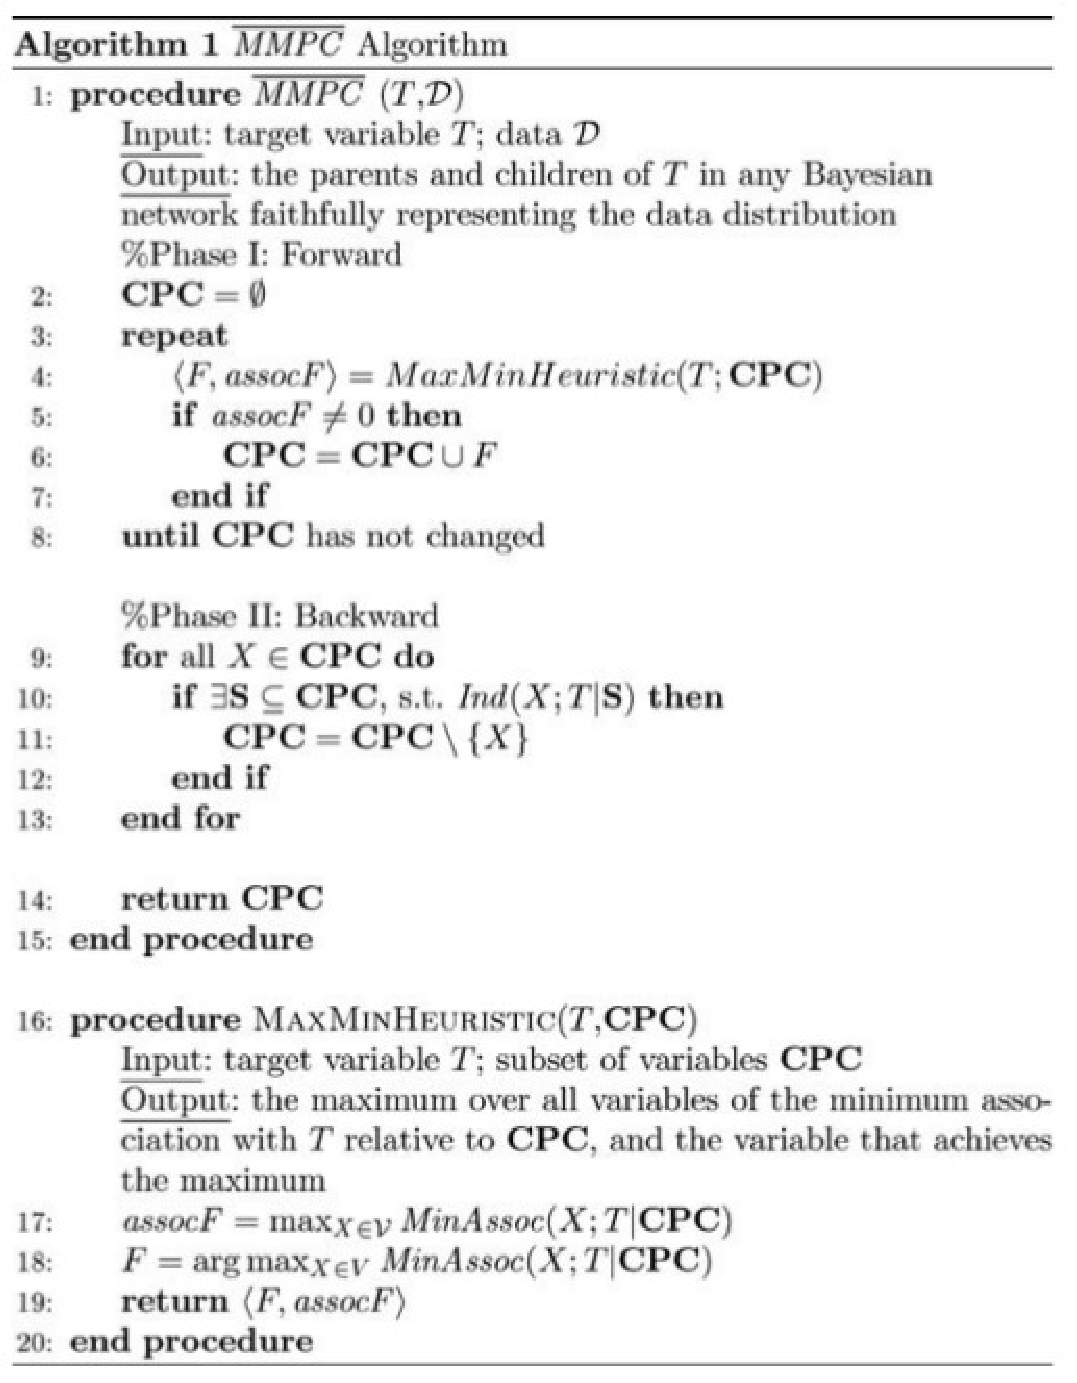
\includegraphics[scale=0.38]{img/mmpc_bar}
				\end{figure}
			\end{center}
		\end{frame}
	\end{center}

\section{Backward phase}
	\begin{center}
		\begin{frame}
			\begin{center}
				\begin{figure}
					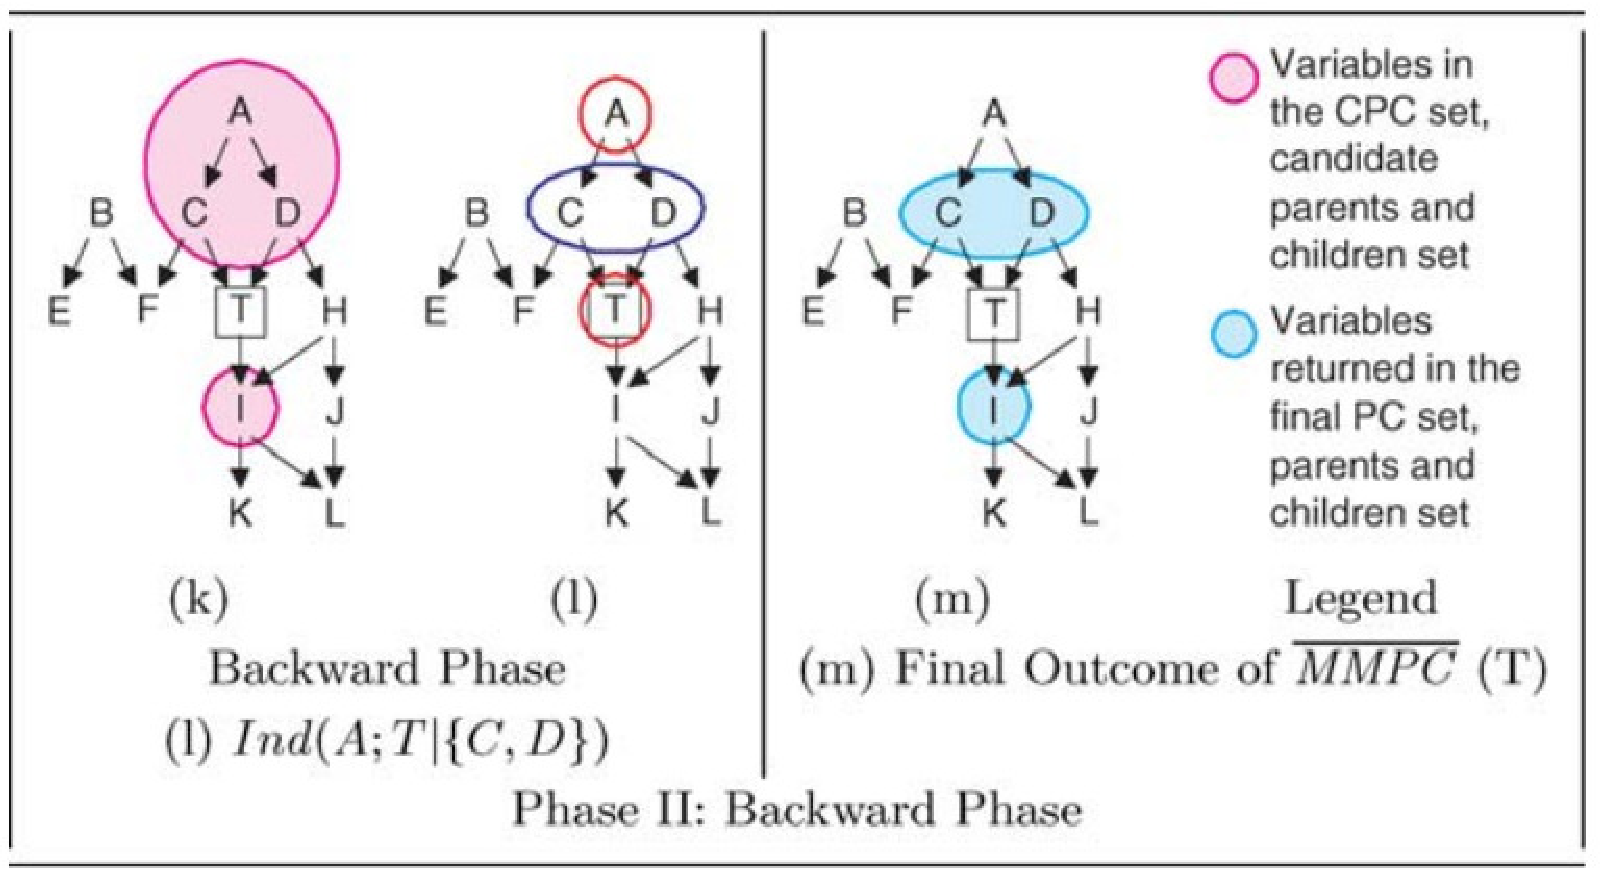
\includegraphics[scale=0.3]{img/backward}
				\end{figure}
			\end{center}
		\end{frame}
	\end{center}

\section{What's next?}
	\begin{frame}
			\frametitle{The last goal:}
				$
					\psmatrix[colsep=1.2cm,rowsep=1cm,mnode=circle]
					&Difficulty&&Intelligence\\
					&&Grade&&SAT\\
					&&Letter
					\ncline{->}{1,2}{2,3}
					\ncline{->}{1,4}{2,3}
					\ncline{->}{1,4}{2,5}
					\ncline{->}{2,3}{3,3}
					\endpsmatrix
				$
		\end{frame}

\section{Thank you}
	\begin{frame}
		$
			\psmatrix[colsep=1.2cm,rowsep=1cm,mnode=circle]
			&Thank&&you\\
			&&for&&your\\
			&&attention
			\ncline{->}{1,2}{1,4}
			\ncline{->}{1,4}{2,3}
			\ncline{->}{2,3}{2,5}
			\ncline{->}{2,5}{3,3}
			\endpsmatrix
		$
	\end{frame}

\end{document}